\documentclass[thesis.tex]{subfiles}

\chapter{Results and Evaluation}
\section{Experiment Setup}
To benchmark BK.Synpase's performance, we trained the presented RetinaNet architecture using the framework. The RetinaNet implementation is written in PyTorch, based on an open source implementation and slightly modified to run on both CPU and GPU for testing purposes. The modified code is available at:\\
\href{https://github.com/lanPN85/pytorch-retinanet-1}{https://github.com/lanPN85/pytorch-retinanet-1}

Due to resource constraints, we were only able to test the system on a small 2-machine setup. Both machine runs on Ubuntu Linux 18.04, which we denote as N1 and N2. They are connected via an Ethernet connection over a 100Mbps network switch. The shared data folder is on an HDD drive physically connected to N1, and mounted on N2 using Linux NFS mount. Each machine runs a BK.Synapse node daemon, while N2 also hosts the API server and the web application (Figure \ref{fig:deployment}).

\begin{table}[]
    \caption{Hardware specifications for nodes N1 and N2}
    \centering
    \begin{tabu} to \textwidth {|c|X[c]|X[c]|}
        \hline
        \textbf{Component} & \textbf{N1} & \textbf{N2} \\ \hline
        CPU & Intel Core i7-8700K, 3.70GHz & Intel Core i7-6700K, 4.00GHz \\ \hline
        CPU Cores & 6 & 4 \\ \hline
        RAM & 64GB & 32GB \\ \hline
        GPU & NVIDIA GeForce GTX 1080Ti & NVIDIA GeForce GTX 1080 \\ \hline
        GPU Memory & 12GB & 8GB \\ \hline
    \end{tabu}
    \label{tab:n1n2_specs}
\end{table}

\begin{figure}[htp]
	\centering
	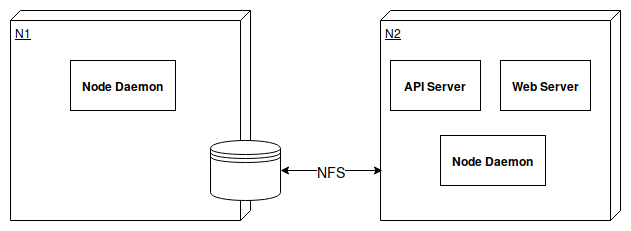
\includegraphics[width=0.9\textwidth]{deployment.png}
	\caption{Deployment diagram for our experiments}
	\label{fig:deployment}
\end{figure}
% \FloatBarrier

The training and test datasets are from ICDAR 2019 RobustReading Challenge on Scanned Receipts OCR and Information Extraction, Task 1\footnote{http://rrc.cvc.uab.es/?ch=13}. The original dataset consists of 626 images of scanned receipts, with annotations for invidual text block positions and their content. We split this data into 532 images for the train set, 47 images for the validation set and 47 images for the test set. While the original challenge is to both locate each block and predict their content, we focus solely on the task of locating blocks using RetinaNet.

\begin{figure}[htp]
	\centering
	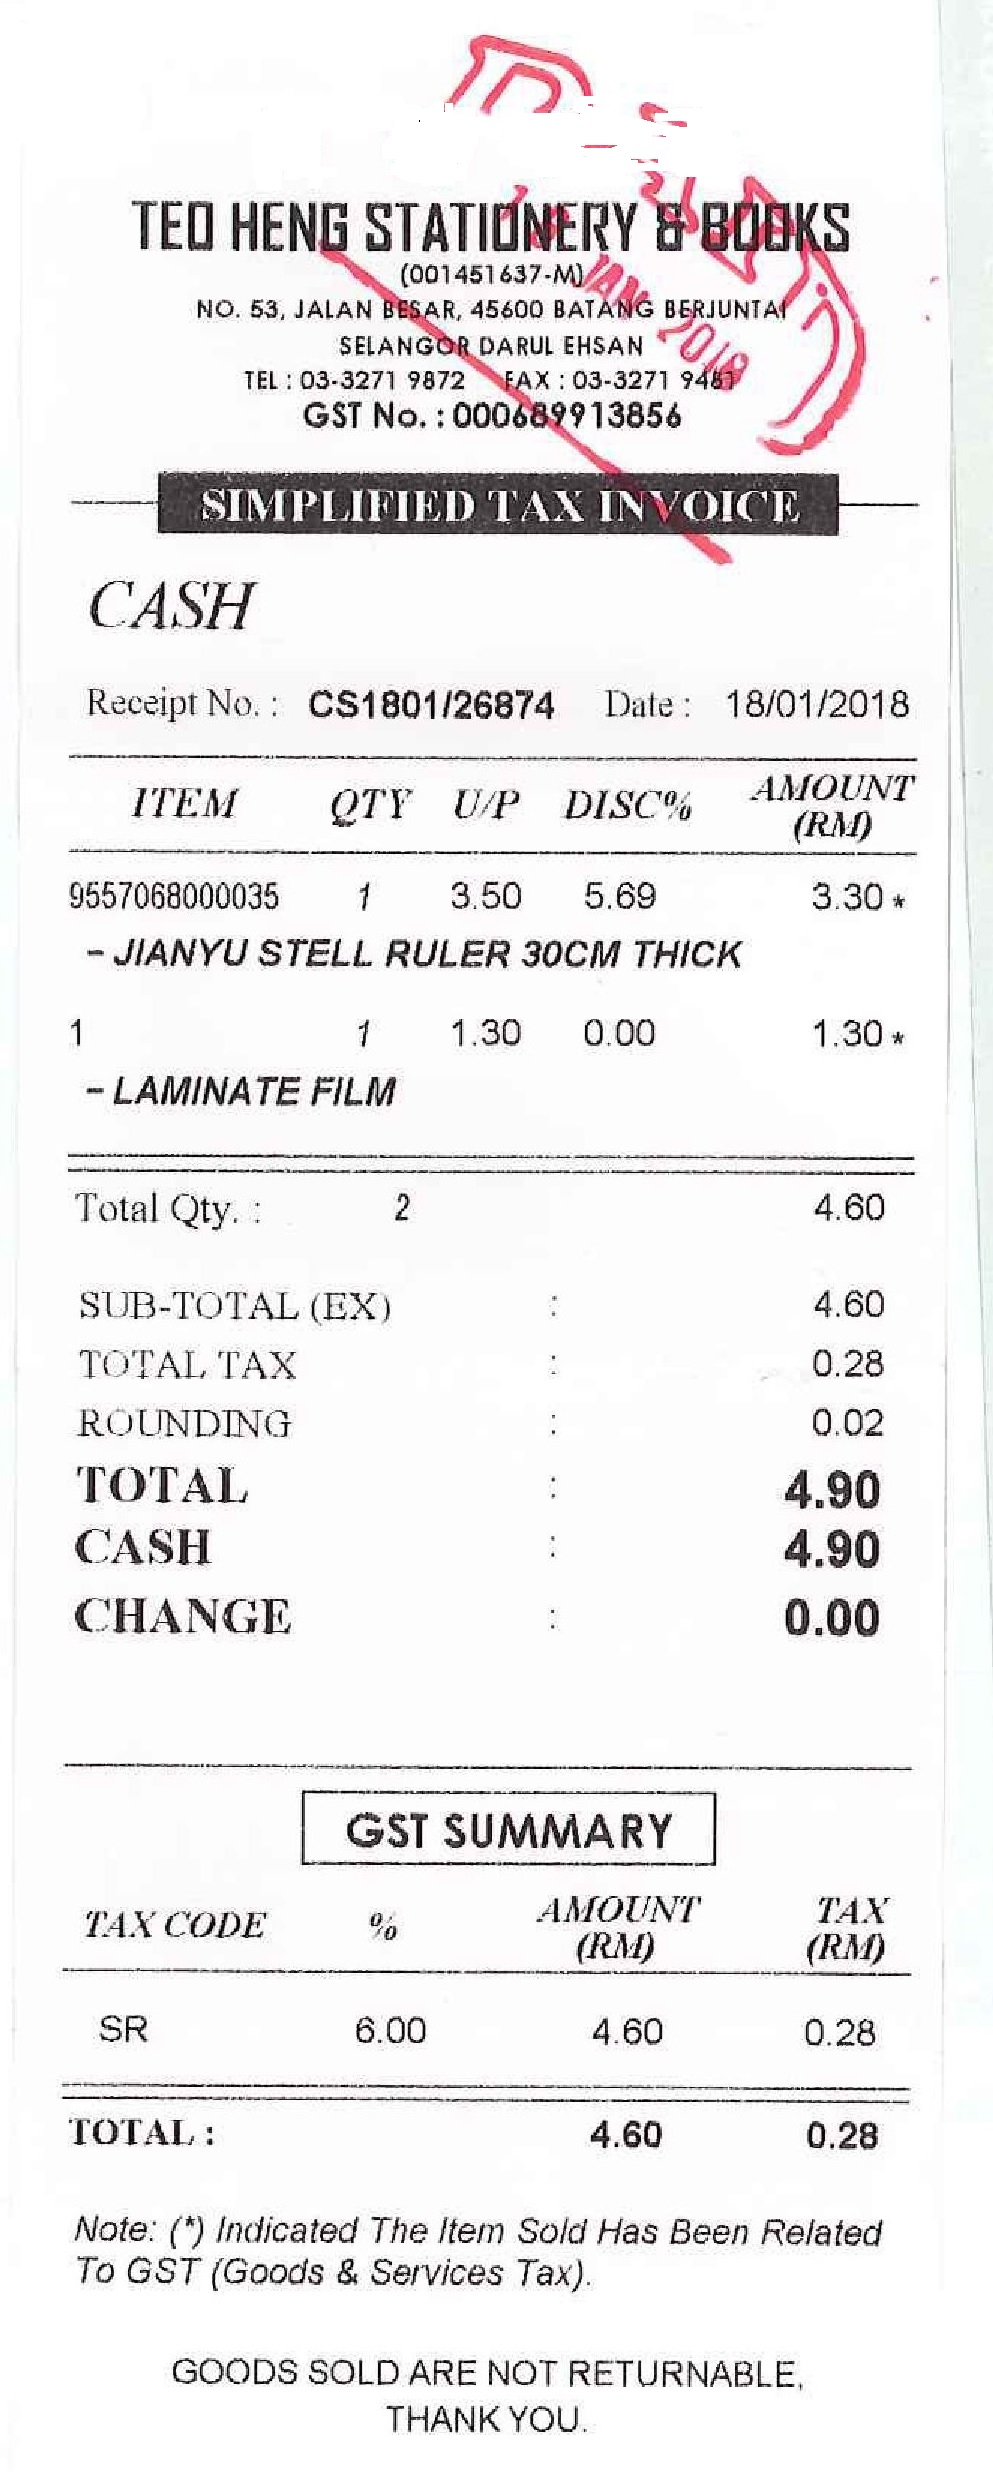
\includegraphics[width=0.2\textwidth]{data_example.jpg}
	\caption{An example scanned receipt from the ICDAR Challenge dataset}
	\label{fig:data_example}
\end{figure}

\section{Training Benchmarks}
Our first set of experiments seek to benchmark BK.Synapse's performance when training a large, production-level architecture. We trained the network with 4 different resource configurations: 1 CPU, 2 CPUs, 1 GPU, and 2 GPUs. The training configurations for each run are identical as shown in Table \ref{tab:train_params}.

\begin{table}[]
\centering
\caption{Benchmark training configuration}
\begin{tabu} to 0.8\textwidth {|X[c]|X[c]|}
    \hline
    \textbf{Parameter} & \textbf{Value} \\ \hline
    Network backbone & ResNet-50 \\ \hline
    Learning rate & 0.001 \\ \hline
    Batch size & 2 \\ \hline
    Gradient norm & 0.1 \\ \hline
    No. epochs & 10 \\ \hline
    Snapshot frequency & 2 \\ \hline
\end{tabu}
\label{tab:train_params}
\end{table}
\FloatBarrier

The listed batch size (2) is the per-node batch size. This value is quite smaller than normal, due to the size of the network and the input images. We find that a batch size of 2 avoids out-of-memory errors for our GPUs.

This benchmark is primarily concerned with parallelization metrics, including speedup and efficiency when training with multiple CPUs/GPUs, as shown in Table \ref{tab:benchmarks}. We measure the average time in seconds for each epoch and step for comparison. Speedup and efficiency are measured using per epoch time.

\begin{table}[]
    \caption{Benchmark time, speedup ratio and efficiency index for training RetinaNet in parallel}
    \centering
    \begin{tabu} to \textwidth {|X[c]|c|c|c|c|}
        \hline
        \textbf{Resources} & \textbf{Avg. epoch time} & \textbf{Avg. step time} & \textbf{Speedup} & \textbf{Efficiency} \\ \hline
        1 CPU & 2130.33s & 7.92s & - & - \\ \hline
        2 CPUs & 1421.10s & 10.41s & 1.50x & 75.00\% \\ \hline
        1 GPU & 832.79s & 3.04s & - & - \\ \hline
        2 GPUs & 606.14s & 4.48s & 1.37x & 68.70\% \\ \hline
    \end{tabu}
    \label{tab:benchmarks}
\end{table}

As the 2CPUs/2GPUs setups work with larger batches, we see an increase in the average step time compared to single-node setups. For CPU runs, step time increases from 7.92s to 10.41s, whereas GPU runs increase from 3.04s to 4.48s. However, since epochs are now shorter, the overall epoch time is sped up. ON average, a CPU epoch decreases by approximately 700s (11 minutes), and a GPU epoch decreases by 200s (3 minutes). a On 2 GPUs, BK.Synapse achieves a somewhat average efficiency index of 68.70\%. On 2 CPUs, efficiency is slightly higher at 75.00\%. This leaves quite some room for improvements, especially in terms of framework-specific tasks like logging and monitoring. However, the training speedup is still significant, and can be very useful in practice. Figure \ref{fig:epochs_chart} shows the average epoch time between these configurations and the "ideal" runtime (ie. efficiency equals 100\%).

\begin{figure}[htp]
	\centering
	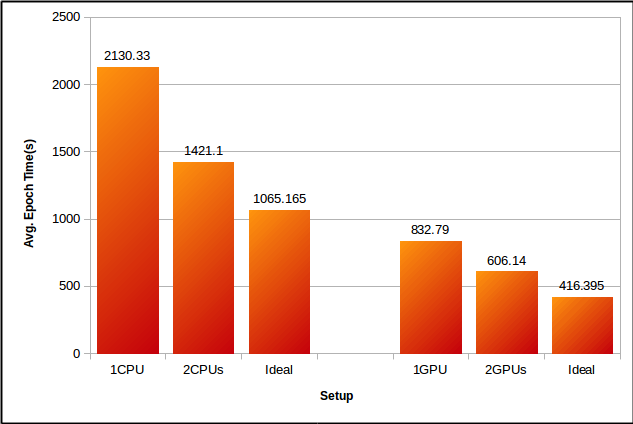
\includegraphics[width=0.75\textwidth]{epochs_chart.png}
	\caption{Average epoch time for different parallel configurations}
	\label{fig:epochs_chart}
\end{figure}
\FloatBarrier

\section{Model Performance}
In our final experiment, we train the same network to convergence using BK.Synapse, and evaluate the final model's performance on the \gls{icdar} Challenge task. We maintain the same parameters as in Table \ref{tab:train_params}, while the number of epochs is set to 100. The networks are trained on both N1 and N2 with GPU acceleration.

We sample 3 different values of $\gamma$ for Focal Loss: 0.5, 1.0, and 2.0. \gls{ap} at IoU=0.5 and IoU=0.75 are used as our evaluation metrics. The final training results are shown in Table \ref{tab:ap}.

\begin{table}[]
    \centering
    \caption{Average precision at IoU=0.5 and IoU=0.75 for different values of $\gamma$}
    \begin{tabu} to \textwidth {|c|X[c]|X[c]|X[c]|X[c]|X[c]|X[c]|}
        \hline
         & \multicolumn{3}{c|}{\textbf{AP@0.50}} & \multicolumn{3}{c|}{\textbf{AP@0.75}} \\ \cline{2-7}
         & \textbf{Train set} & \textbf{Val set} & \textbf{Test set} & \textbf{Train set} & \textbf{Val set} & \textbf{Test set} \\ \hline
        $\gamma = 0.5$ & - & - & - & - & - & - \\ \hline
        $\gamma = 1.0$ & - & - & - & - & - & - \\ \hline
        $\gamma = 2.0$ & - & - & - & - & - & - \\ \hline
    \end{tabu}
    \label{tab:ap}
\end{table}

The best model's loss values (regression and classification loss) at each epoch for the training and validation sets are shown in Figures \ref{fig:train_loss}, \ref{fig:val_loss} and \ref{fig:cmp_loss}.

\begin{figure}[htp]
	\centering
	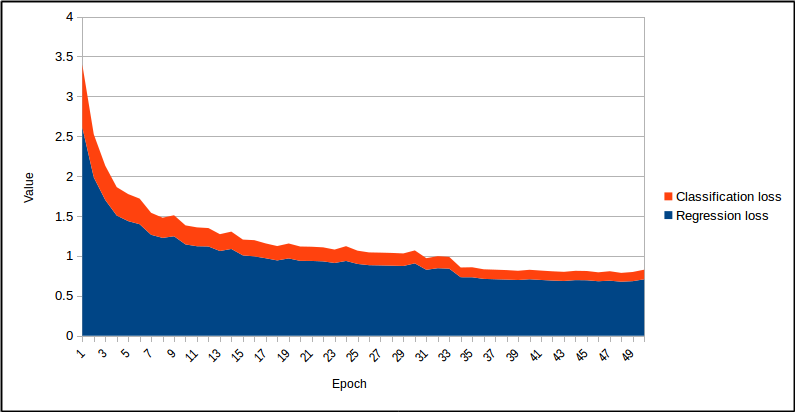
\includegraphics[width=0.9\textwidth]{train_loss.png}
	\caption{Regression loss and classification loss over epochs on the training set}
	\label{fig:train_loss}
\end{figure}

\begin{figure}[htp]
	\centering
	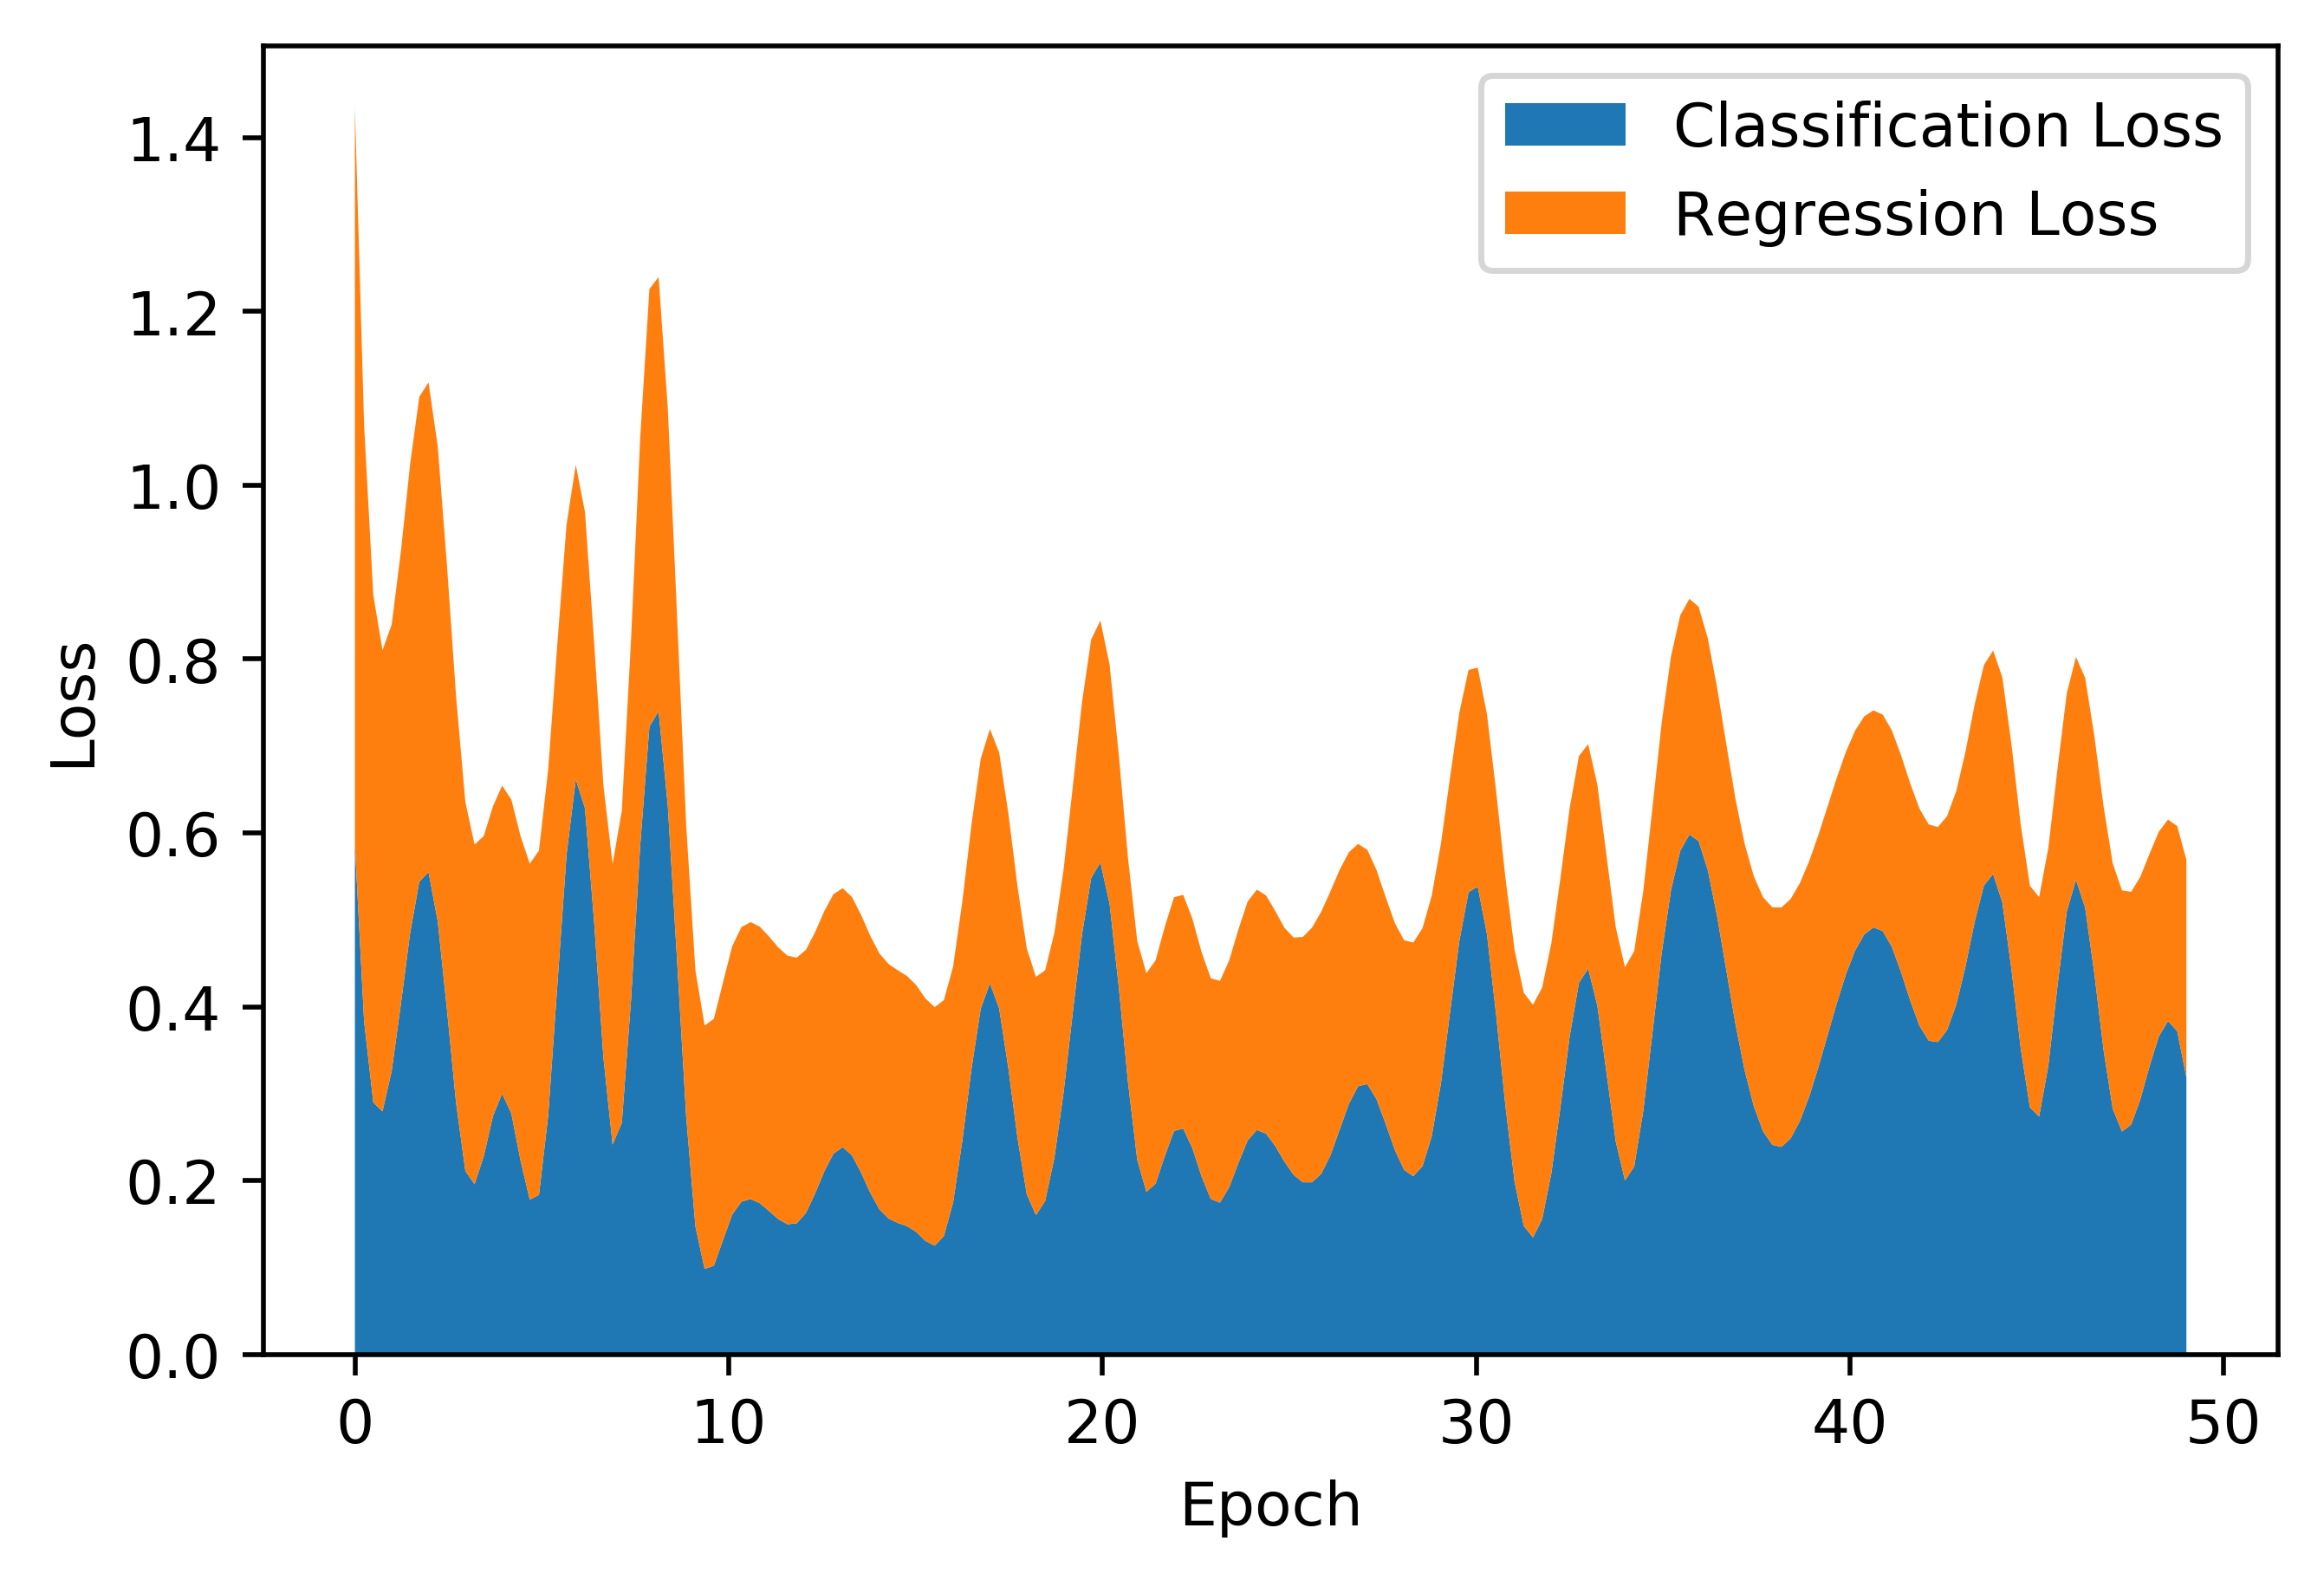
\includegraphics[width=0.9\textwidth]{val_loss.png}
	\caption{Regression loss and classification loss over epochs on the validation set}
	\label{fig:val_loss}
\end{figure}

\begin{figure}[htp]
	\centering
	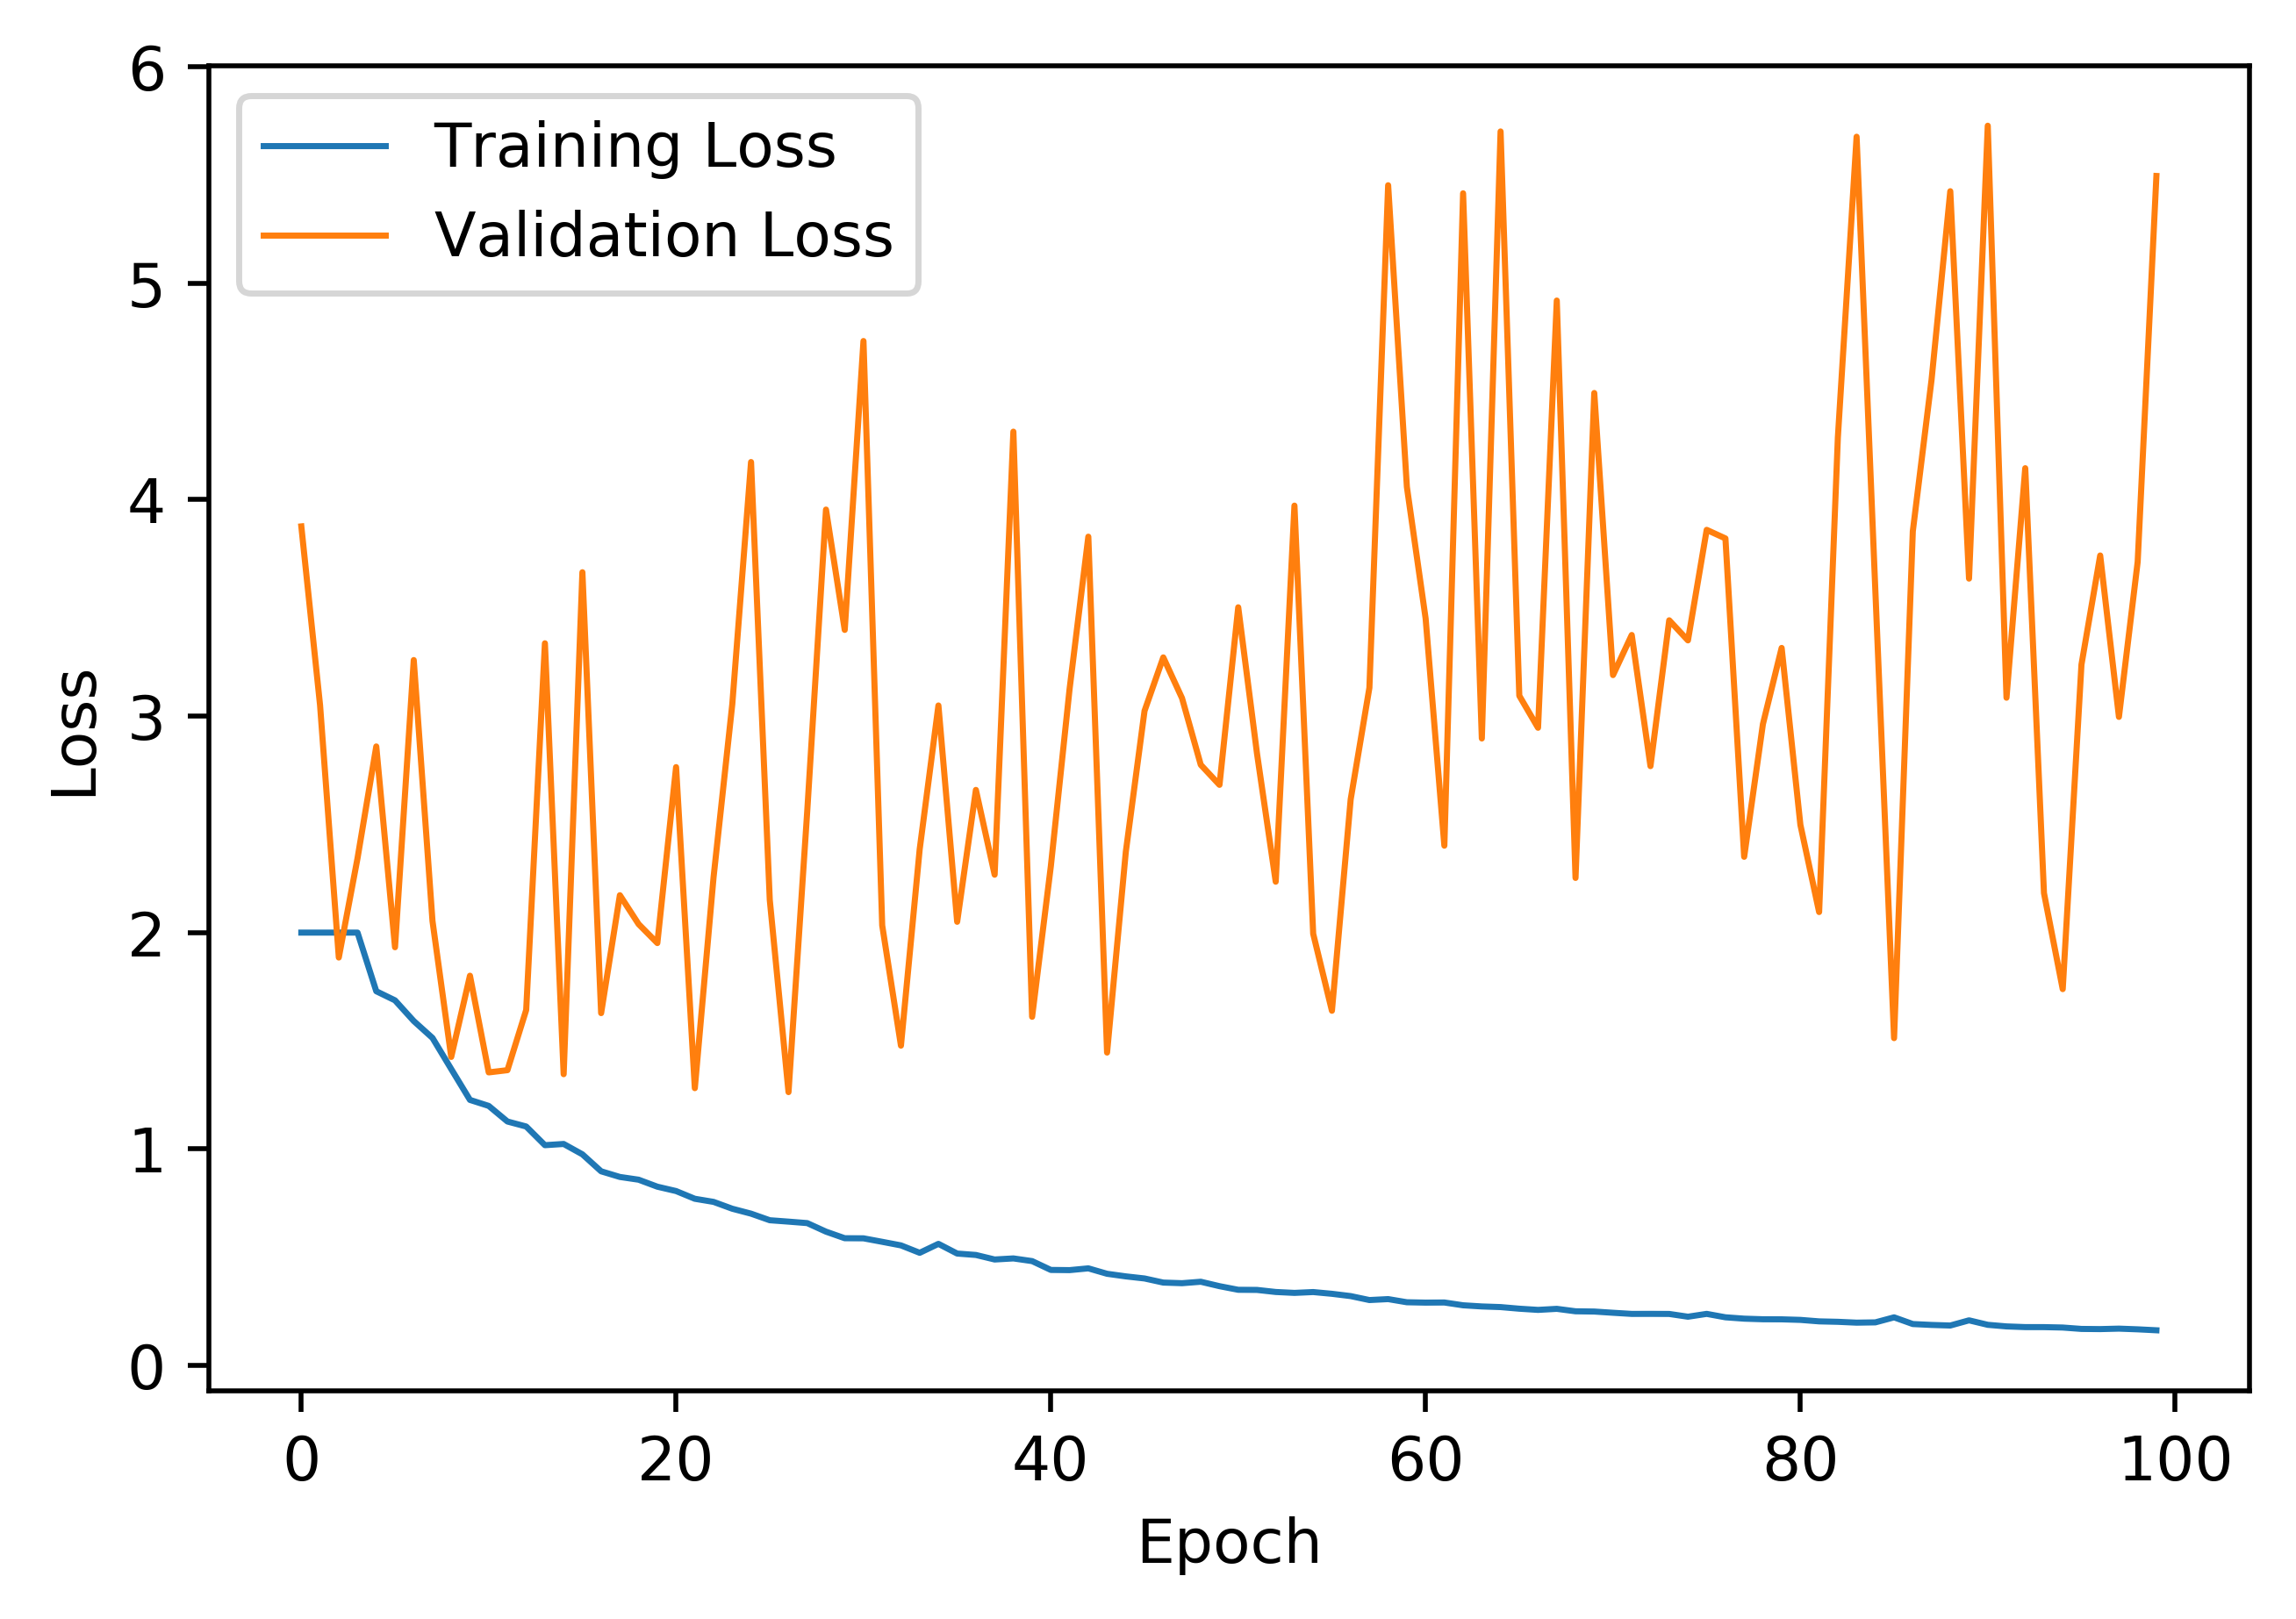
\includegraphics[width=0.9\textwidth]{cmp_loss.png}
	\caption{Loss value comparison between the training and validation set}
	\label{fig:cmp_loss}
\end{figure}

The loss values implies slight overfitting, and shows with a final \gls{ap} gap of ???. This can be partially attributed to the small training dataset with high example variance. Regardless, the model performs reasonably well on our test examples, with a test \gls{ap} of ???. Further adjustments can be made to better adapt RetinaNet to text boxes, however we will not go into further detail in this case study.
